%! Author = matteomagnini
%! Date = 05/03/25

%----------------------------------------------------------------------------------------
\chapter{Neuro-symbolic AI}
\label{ch:nesy-ai}
\minitoc
%----------------------------------------------------------------------------------------

\section[Symbolic knowledge injection]{\Glsentrylong{SKI}}\label{sec:ski}
%
\Gls{SKI} is a wide sub-field of \gls{NeSy}, which encompasses all the methods that in some way \emph{inject} symbolic knowledge into sub-symbolic predictors.
%
More precisely, we define \gls{SKI} as:
%
\begin{definition}[\gls{SKI}]
    \label{def:ski}
    any \textbf{algorithmic} procedure affecting how sub-symbolic predictors draw their inferences in such a way that predictions are either \textbf{computed} as a function of, or made \textbf{consistent} with, some given symbolic knowledge~\cite{DBLP:journals/csur/CiattoSAMO24}.
\end{definition}
%
We adopt this broad definition because the amount of works in the literature is vast and varied, furthermore the contributions come from different communities (e.g., \gls{ML}, \gls{AI}, \gls{NLP}, \gls{XAI}, logics, etc.), and they often use different terminologies.
%
In the rest of this thesis, we will refer to \emph{uneducated predictor} to indicate a sub-symbolic predictor that does not use symbolic knowledge -- i.e., before the injection takes place --, and to \emph{educated predictor} to indicate a sub-symbolic predictor that uses symbolic knowledge---i.e., after the injection takes place.
%
Sometimes, in the literature the term \emph{enriched predictor} is also used instead of \emph{educated predictor}.


\subsection{Motivations and goals}\label{subsec:ski-motivations-and-goals}
%
\Gls{SKI} can be used for several reasons, such as:
%
\begin{inlinelist}
    %
    \item \label{itm:prediction}\emph{improving the model's predictive performance}, by leveraging symbolic knowledge to guide their learning or inference;
    %
    \item \label{itm:interpretability}\emph{improving the model's interpretability}, by making their predictions consistent with symbolic knowledge;
    %
    \item \label{itm:robustness}\emph{increase the robustness} of sub-symbolic predictors, by making them less sensitive to data perturbations (e.g., noise, data scarcity, etc.);
    %
    \item \label{itm:complexity}\emph{reduce the model complexity} of the models, by shaping their structure or by constraining their parameters;
    %
    \item and possibly many more.
    %
\end{inlinelist}


\Cref{itm:prediction} is one of the most common motivations for \gls{SKI}.
%
The idea is simple: if there is already some (symbolic) knowledge about a particular domain or task, then it is reasonable to expect that the predictor can benefit from it.
%
In this way the model learns both from the data -- inductively -- and from the symbolic knowledge---mimicking deductive reasoning.


Another common reason to use \gls{SKI} is to increase the \emph{interpretability} of the model, as stated in \Cref{itm:interpretability}.
%
In the context of \gls{XAI}, this is usually referred as \gls{XAI} \emph{by design} (\Cref{par:xai-by-design}).
%
The intuition is simple: the model is made to be consistent -- up to a certain extent -- with the symbolic knowledge, which is usually more interpretable than the model itself.
%
This can be done in two ways: either by using \emph{symbols as constraints} or by \emph{transparent box design}.
%
More details about these two approaches are provided in \Cref{subsec:learning} and \Cref{subsec:structuring}, respectively.


Predictive performances and \gls{XAI} are the main motivations for \gls{SKI}, but not the only ones.
%
The \emph{robustness} (\Cref{itm:robustness}) of a predictive model is another important challenge~\cite{DBLP:conf/eccv/LiuCZH18}, and it relates to predictors' ability to maintain performance despite the presence of input perturbations.
%
A metric of robustness in the context of \gls{SKI} is defined in the work ``An Empirical Study on the Robustness of Knowledge Injection Techniques Against Data Degradation''~\cite{DBLP:conf/woa/RafanelliMACO24}.
%
The content of the paper is presented in~\Cref{subsec:empirical-study-on-the-robustness-of-ski-methods}.
%
Along with robustness, there are other metrics -- often neglected -- that play a crucial role in the design of intelligent systems, such as \emph{memory footprint} (\Cref{itm:complexity}), \emph{latency}, data efficiency, and so on.
%
These \gls{QoS} metrics are presented in the work ``Symbolic Knowledge Injection Meets Intelligent Agents: QoS metrics and experiments''~\cite{DBLP:journals/aamas/AgiolloRMCO23}, which is discussed in~\Cref{subsec:ski-meets-intelligent-agents}.


\subsection{What to inject}\label{subsec:what-to-inject}
%
\begin{SCfigure}
    \centering
    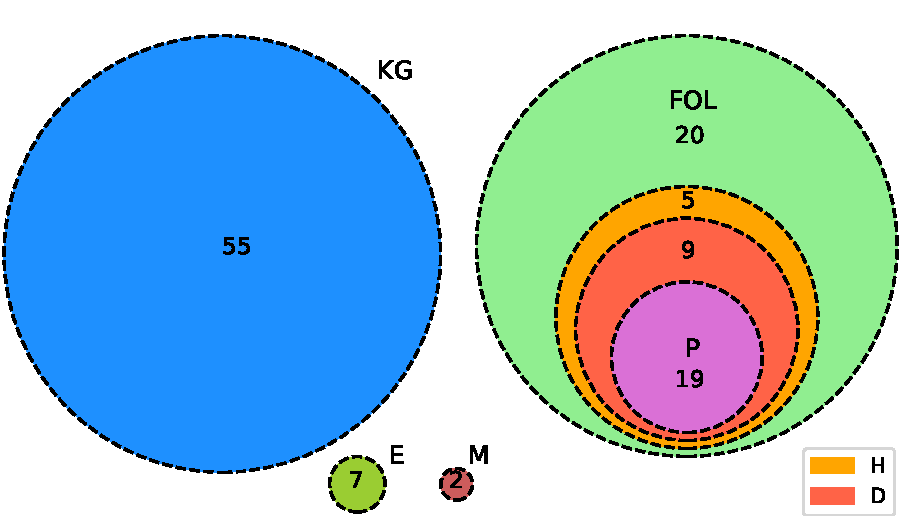
\includegraphics[width=.4\linewidth]{figures/ski-logic}
    \caption[Venn diagram categorising SKI methods]{
        Venn diagram categorising SKI methods w.r.t.\ the \emph{input knowledge} type: knowledge graphs (KG), propositional logic (P), first-order logic (FOL), expert knowledge (E), Datalog (D), Horn logic (H), or modal logic (M).
        %
        The image is taken from~\cite{DBLP:journals/csur/CiattoSAMO24} and it refers to 117 surveyed \gls{SKI} methods.
    }
    \label{fig:pie-ski-logic}
\end{SCfigure}

%
A key distinction in \gls{SKI} methods lies in whether the chosen formalism is \emph{machine interpretable}, \emph{human interpretable}, or both.
%
\Gls{SKI} methods can be categorized into two primary groups based on the formalism used to represent input knowledge~\cite{DBLP:journals/csur/CiattoSAMO24}:
%
\begin{itemize}
    \item \textbf{Logic formulas or \glspl{KB}:} These adhere to \gls{FOL} or its subsets, making them interpretable by both humans and machines.
    %
    The sub-categories, ordered by decreasing expressiveness, include:
    %
    \begin{itemize}
        %
        \item \emph{\gls{FOL} formulas:} These encompass recursive terms, variables, predicates of any arity, and various logic connectives, potentially expressing definitions.
        %
        \item \emph{Horn logic:} Often referred to as Prolog-like logic, this formalism consists of head–body rules involving predicates and terms of any kind.
        %
        \item \emph{Datalog:} A restricted subset of Horn logic that excludes recursive terms, allowing only constants or variables as terms.
        %
        \item \emph{Modal logics:} These extend the above logics with modal operators (e.g., \(\square\) and \(\lozenge\)), which express modalities such as necessity or possibility.
        %
        \item \emph{Knowledge graphs:} A practical application of description logics designed to represent entity–relation graphs.
        %
        \item \emph{Propositional logic:} This involves Boolean variables and logical connectives, offering a simpler yet effective formalism.
    \end{itemize}
    %
    \item \textbf{Expert knowledge:} This category includes human-interpretable knowledge that is not inherently machine-readable.
    %
    Examples include physics equations, syntactical rules, or domain-specific expertise.
    %
    Since expert knowledge is not directly machine interpretable, it often requires transformation into tensorial form through data generation, a process that typically involves human engineers and can be labor-intensive.
\end{itemize}
%
\Cref{fig:pie-ski-logic} illustrates the distribution of surveyed \gls{SKI} methods based on their formalism of choice.
%
\Glspl{KG} emerge as the most prevalent category, representing nearly half of the surveyed methods.
%
In contrast, modal logics constitute the smallest group.
%
Methods based on \gls{FOL} or its subsets (excluding \glspl{KG}) form another significant cluster, with propositional logic being particularly prominent due to its relative simplicity and widespread use.
%
The specific logic formalism employed in the surveyed papers is reported where available.
%
However, this information is rarely explicitly stated by the authors.
%
Instead, the logic is often inferred from the constraints and descriptions provided in the respective works.

Practical examples of symbolic knowledge that can be injected into sub-symbolic predictors are the public health guidelines on type-2 diabetes of the National Institute of Diabetes and Digestive and Kidney Diseases\footnote{\url{https://www.niddk.nih.gov/health-information/diabetes/}}.
%
These guidelines have been encoded into logic formulas~\cite{DBLP:conf/pkdd/KunapuliBSMS10} and used in works related to \gls{SKI}~\cite{Magnini-telmed2025}.
%
The first guideline state that if a patient has a glucose value greater or equal to 125 mg/dL and a \gls{BMI} greater or equal to 30, then the patient is considered diabetic.
%
The second one says that if a patient has a glucose value lower or equal to 100 mg/dL and a \gls{BMI} lower or equal to 25, then the patient is considered non-diabetic.
%
In \gls{FOL}, the first statement can be encoded as:
%
\begin{equation}\label{eq:rule-diabetic}
  \forall x . ( \text{glucose}(x) \geq 125 \land \text{bmi}(x) \geq 30 \rightarrow \text{Diabetic}(x))
\end{equation}
%
whereas the second statement can be encoded as:
%
\begin{equation}\label{eq:rule-not-diabetic}
  \forall x . ( \text{glucose}(x) \leq 100 \land \text{bmi}(x) \leq 25 \rightarrow \neg \text{Diabetic}(x))
\end{equation}


\subsection{How to inject}\label{subsec:how-to-inject}
%
\begin{SCfigure}
    \centering
    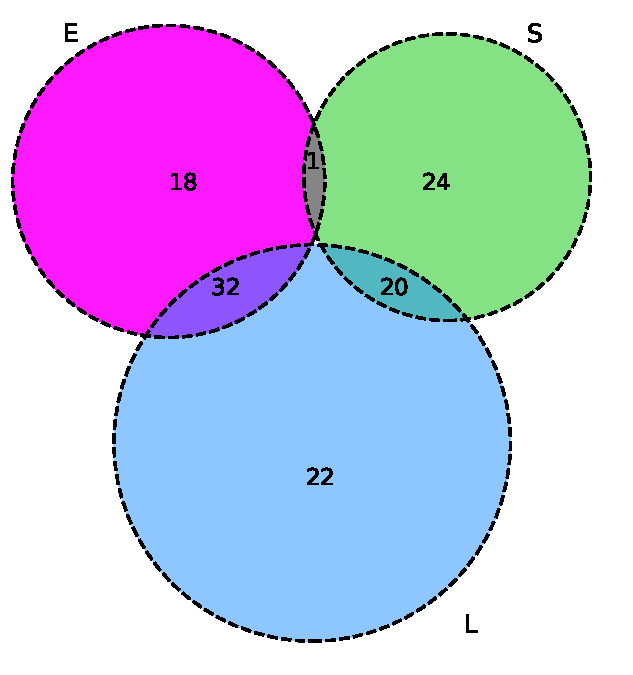
\includegraphics[width=.4\linewidth]{figures/ski-integration}
    \caption[Venn diagram categorising SKI methods]{
        Venn diagram categorising SKI methods w.r.t.\ the \emph{injection} strategy type: structuring (S), embedding (E), or guided learning (L).
        %
        The image is taken from~\cite{DBLP:journals/csur/CiattoSAMO24} and it refers to 117 surveyed \gls{SKI} methods.
    }
    \label{fig:pie-ski-injection}
\end{SCfigure}
%
How can symbolic knowledge, such as the ones in \Cref{eq:rule-diabetic,eq:rule-not-diabetic}, be injected into sub-symbolic predictors?
%
To answer this question, scientists have designed several strategies, which can be broadly grouped into three main categories~\cite{DBLP:journals/csur/CiattoSAMO24}: structuring, guided learning, and embedding.
%
It may occur that a method uses more than one strategy at a time.
%
\Cref{fig:pie-ski-injection} illustrates the distribution of surveyed \gls{SKI} methods based on their strategy of choice.
%
The survey revealed that all three strategies are widely used, with learning being the most frequent but not dominant.

The main entities involved in the \gls{SKI} process -- and that are common to virtually all \gls{SKI} methods -- are:
%
\begin{itemize}
    %
    \item \textbf{symbolic knowledge:} in the vast majority of cases, this is a set of logic formulas or a \gls{KB} that encodes the symbolic knowledge to be injected;
    %
    \item \textbf{parsed knowledge:} a syntactic structure that represents the \emph{parsed} symbolic knowledge, often in the form of a \gls{AST} or graph;
    %
    \item \textbf{sub-symbolic component:} a sub-symbolic instance built upon the parsed symbolic knowledge;
    %
    \item \textbf{uneducated sub-symbolic predictor:} a sub-symbolic predictor that has not been enriched with the symbolic knowledge;
    %
    \item \textbf{educated sub-symbolic predictor:} the final sub-symbolic predictor that has been enriched with the symbolic knowledge.
    %
\end{itemize}
%


\paragraph{Structuring}\label{par:structuring}
%
\begin{figure}
    \centering
    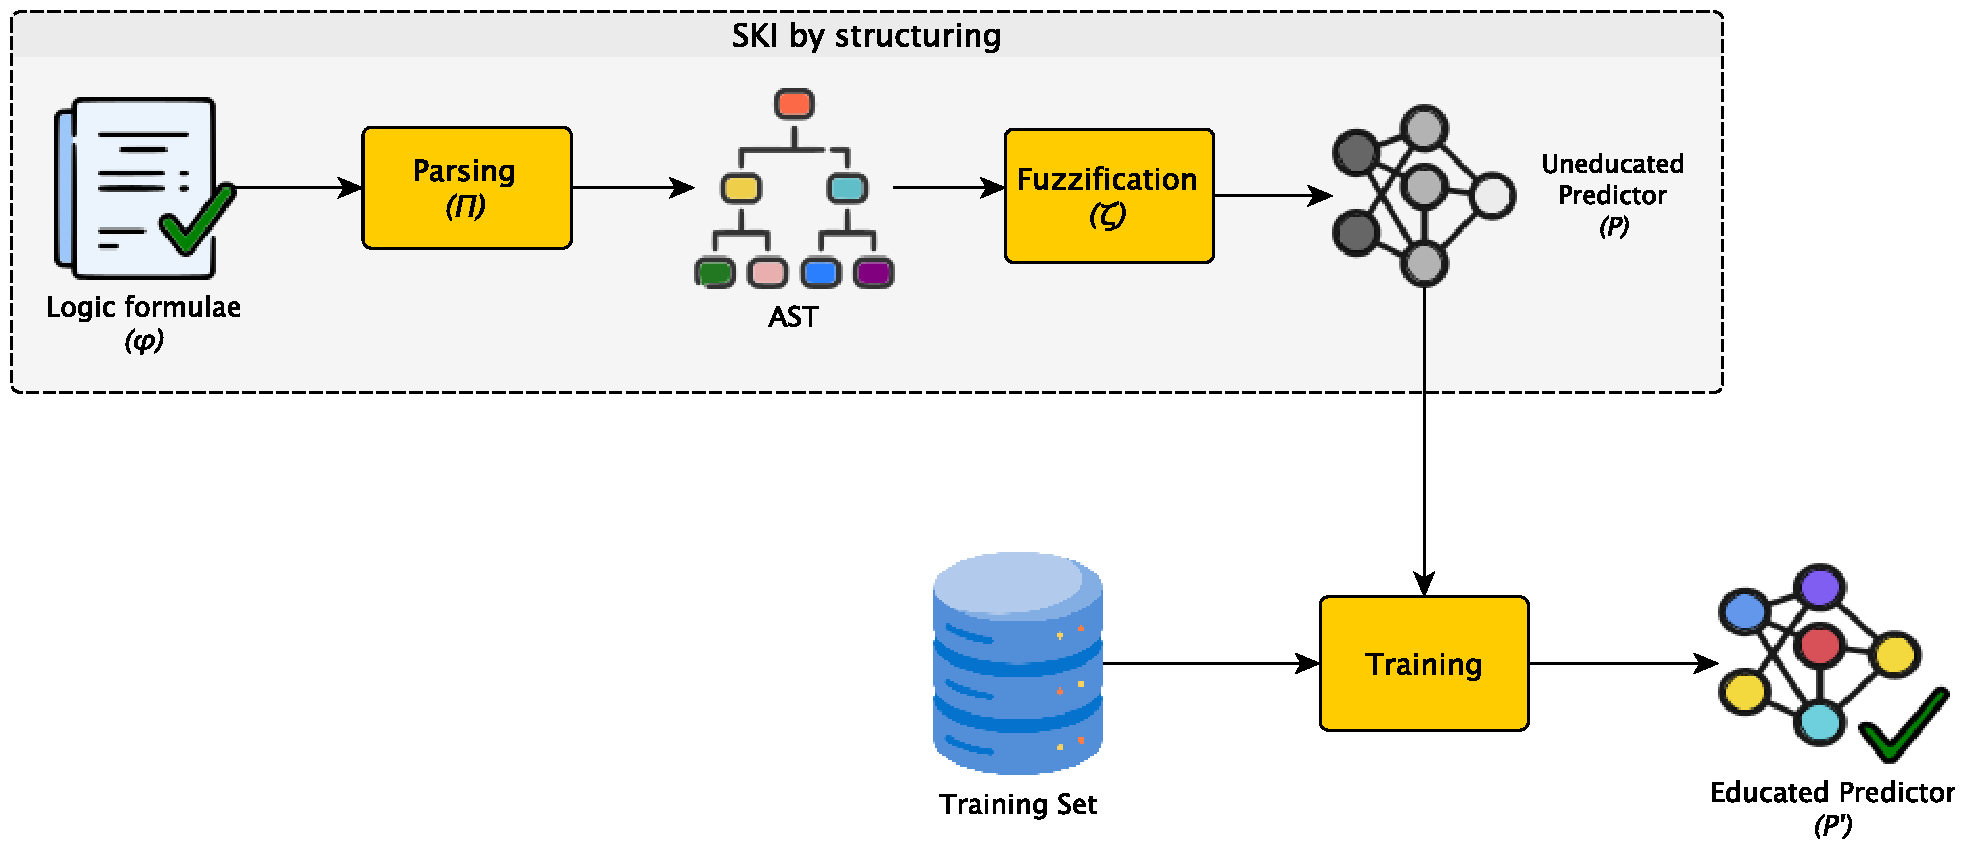
\includegraphics[width=.9\linewidth]{figures/workflow-structuring}
    \caption[SKI workflow of structuring strategy]{
        Workflow of the structuring strategy.
        %
        The symbolic knowledge is parsed and used to create a sub-symbolic predictor -- or part of it -- that mimics the symbolic knowledge.
        %
        The resulting predictor is then trained on data, if needed.
    }
    \label{fig:workflow-structuring}
\end{figure}
%
By predictor structuring, or simply structuring, we identify all those methods that use a part (or the whole) of a sub-symbolic predictor to \emph{mirror} the symbolic knowledge via its own internal structure.
%
A predictor is either created or extended to mimic the behavior of the symbolic knowledge.
%
For instance, when the predictors are \glspl{NN}, their internal structure is crafted to represent logic predicates via neurons, and logic connectives via synapses.
%
\Cref{fig:workflow-structuring} illustrates the workflow of the structuring strategy.
%
Usually, in the structuring strategy, the symbolic knowledge is in the form of logic formulas ($\phi$) (e.g., subsets of \gls{FOL}).
%
The formulas are then parsed into a syntactic structure (e.g., \gls{AST}).
%
At this point, a \emph{fuzzification} ($\zeta$) step is performed to convert the \emph{boolean} (also the term \emph{crisp} is used in the literature) -- because a logic predicate is either \emph{true} or \emph{false} -- symbolic knowledge into a \emph{fuzzy} interpretation of it, which is more suitable for sub-symbolic predictors.
%
This fuzzy interpretation is often \emph{continuous} and bounded to a predefined range, such as \([0, 1]\).
%
The property of continuity is a key requirement for training sub-symbolic structures via gradient descent (e.g., \glspl{NN} or part of them).
%
In practice, $\zeta$ is implemented as a mapping function that transforms logic operators into continuous functions (see \Cref{sec:from-symbolic-to-sub-symbolic}).
%
The result of the fuzzification process is an \emph{uneducated} predictor ($P$) that is then trained on the training set.
%
After the training, the predictor is now \emph{educated} ($P'$) and can be used to make predictions on the test set or in production.
%

\paragraph{Guided learning}\label{par:guided-learning}
%
\begin{figure}
    \centering
    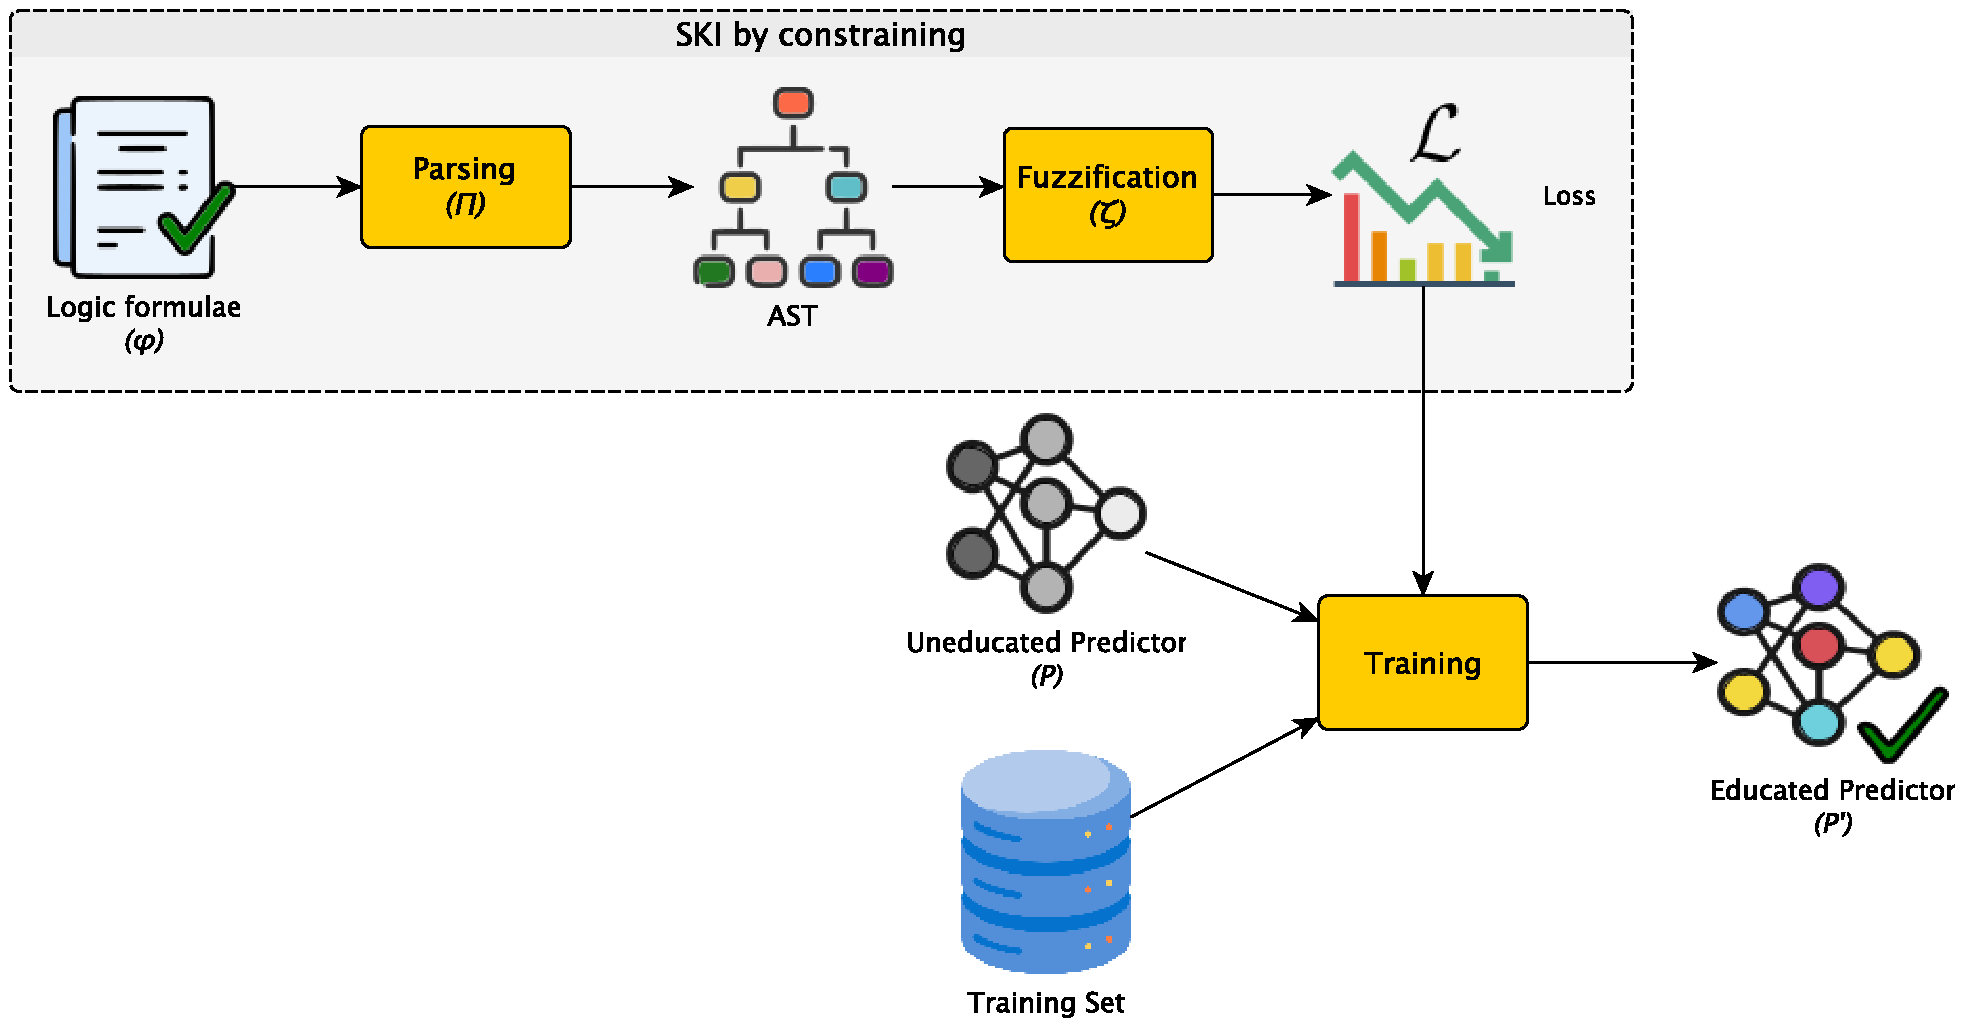
\includegraphics[width=.9\linewidth]{figures/workflow-constraining}
    \caption[SKI workflow of guided learning strategy]{
        \gls{SKI} workflow of the guided learning strategy.
        %
        The symbolic knowledge is used to guide the training of a sub-symbolic predictor, which is then trained on data.
    }
    \label{fig:workflow-learning}
\end{figure}
%
By guided learning, we refer to all those methods that affect the sub-symbolic predictor's training process by using the symbolic knowledge as a \emph{constraint}/\emph{guidance}.
%
Usually, \gls{SKI} algorithms based on this strategy target sub-symbolic predictors that can be trained with gradient descent, such as \glspl{NN}.
%
\Cref{fig:workflow-learning} illustrates the workflow of the guided learning strategy.
%
Like in the case of structuring, the symbolic knowledge is parsed and fuzzified.
%
Differently from structuring, the result of the fuzzification process is not a subcomponent of the predictor's architecture (e.g., neurons, connections), but rather a set of continuous numeric functions.
%
Conceptually, these functions represent the degree of violation of the symbolic knowledge by the predictor's predictions.
%
The higher the degree of violation, the higher the value of the function.
%
The symbolic-derived functions are then included in the loss function of the predictor, which is then trained on the training set.
%
The combination between the ``classical'' loss function (e.g., cross-entropy, mean squared error, etc.) and the symbolic-derived functions can be done in many ways, but it is usually done via a weighted sum.


\paragraph{Embedding}\label{par:ski-embedding}
%
\begin{figure}
    \centering
    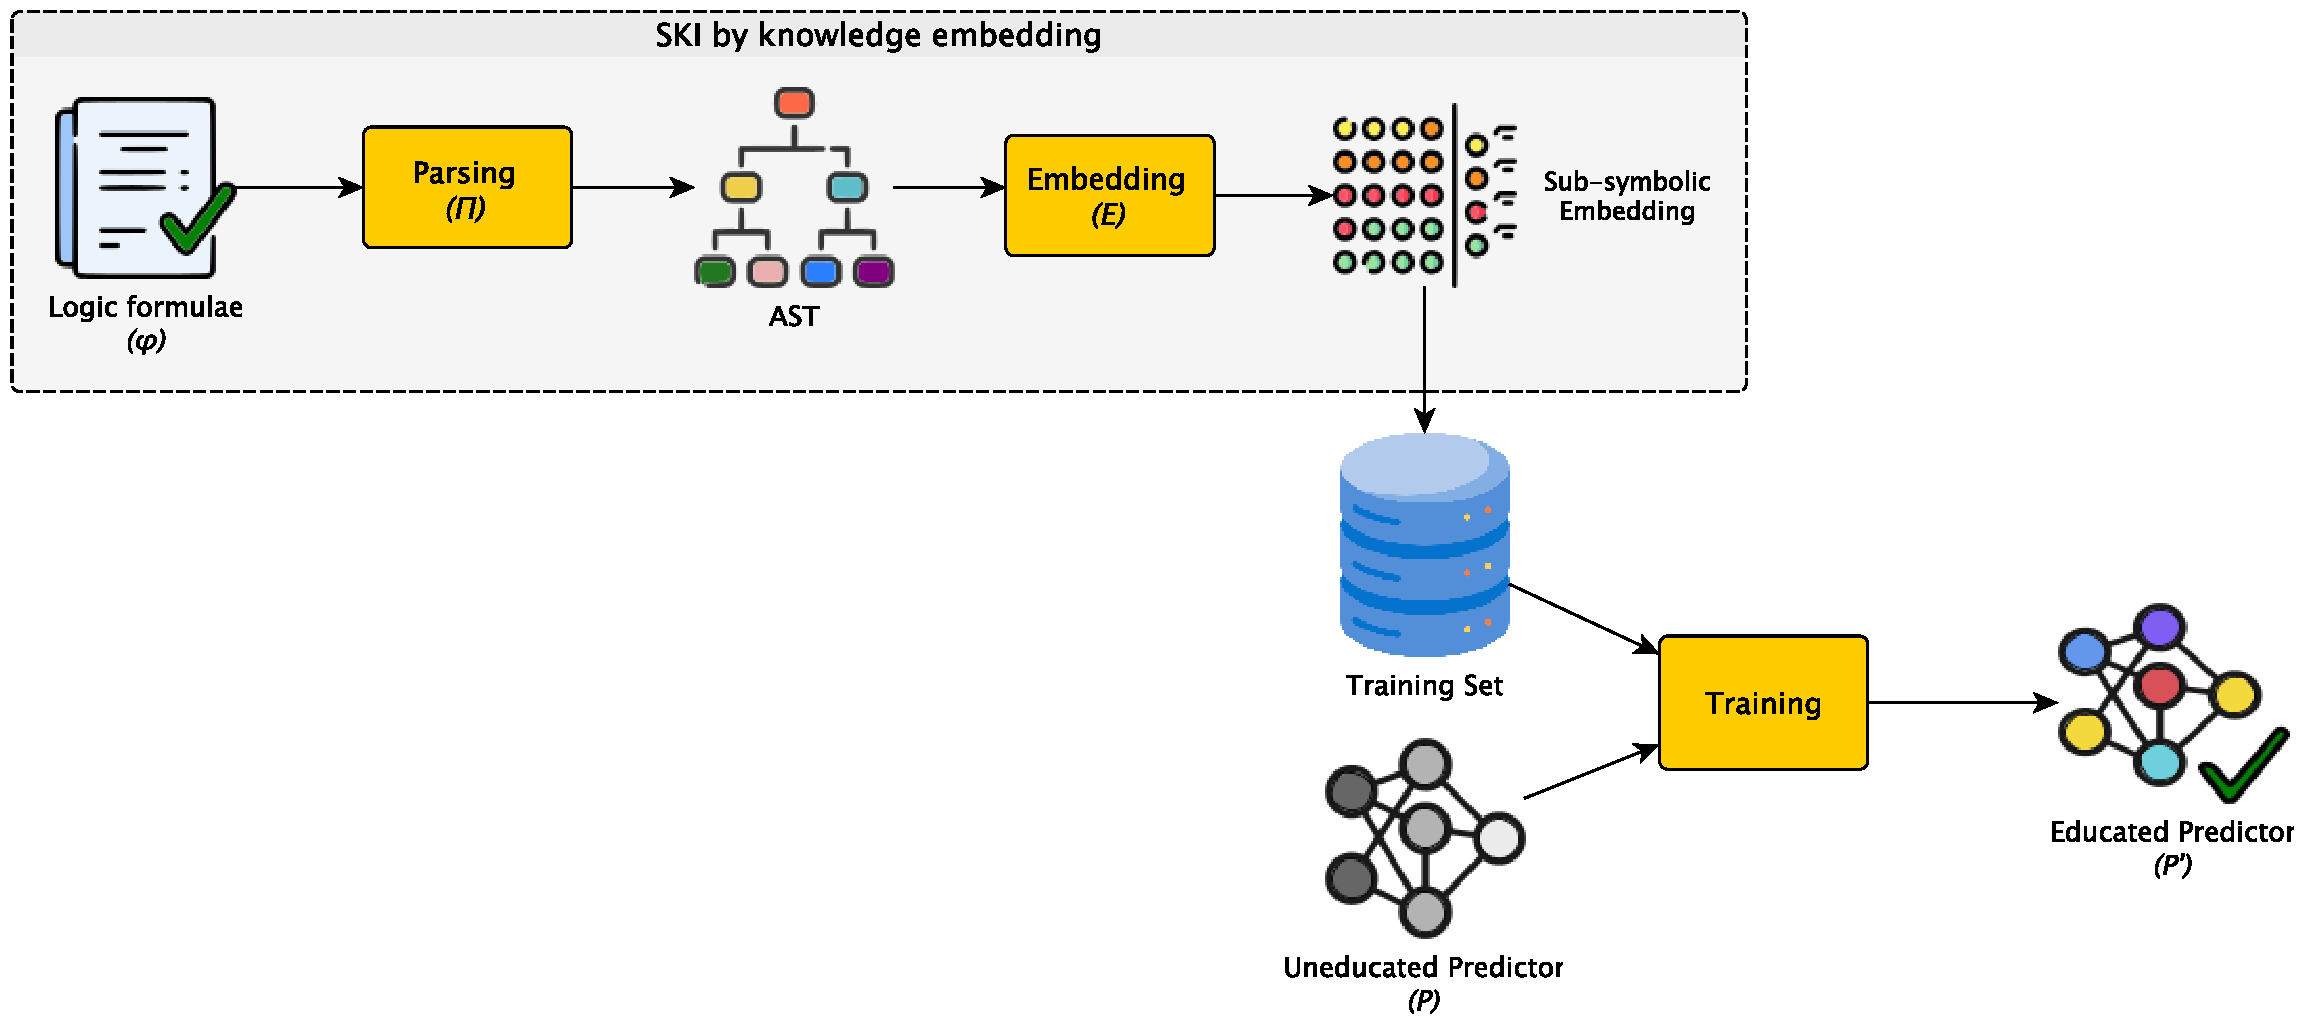
\includegraphics[width=.9\linewidth]{figures/workflow-embedding}
    \caption[SKI workflow of embedding strategy]{
        \gls{SKI} workflow of the embedding strategy.
        %
        The symbolic knowledge is parsed and embedded into a sub-symbolic predictor, which is then trained on data.
    }
    \label{fig:workflow-embedding}
\end{figure}
%
In the embedding strategy, the symbolic knowledge is converted -- i.e., \emph{embedded}-- into numeric-array representations.
%
\Cref{fig:workflow-embedding} illustrates the workflow of the embedding strategy.
%
The output of the fuzzification process is a set of numeric arrays (e.g., vectors, matrices, and tensors) that represent the symbolic knowledge.
%
These arrays are then provided as input to the sub-symbolic predictor.
%
This is the common strategy exploited by the \gls{KG}~\cite{DBLP:conf/ijcai/LambGGPAV20} embedding community as well as by \glspl{GNN}~\cite{DBLP:journals/tkde/WangMWG17}.


\subsection[Limitations and challenges of SKI]{Limitations and challenges of \Gls{SKI}}\label{subsec:limitations-and-challenges-of-ski}


\section[Symbolic knowledge extraction]{\Glsentrylong{SKE}}\label{sec:ske}
%
\gls{SKE} is the process of extracting symbolic knowledge from sub-symbolic predictors.
%
Here, we provide the broad definition of \gls{SKE} that we adopt in this thesis:
%
\begin{definition}[\gls{SKE}]
    \label{def:ske}
    any \textbf{algorithmic} procedure accepting \textbf{trained} sub-symbolic predictors as input and producing \textbf{symbolic} knowledge as output so that the extracted knowledge reflects the behavior of the predictor with high \textbf{fidelity}~\cite{DBLP:journals/csur/CiattoSAMO24}.
\end{definition}
%


\subsection{Motivations and goals}\label{subsec:ske-motivations-and-goals}

\subsection{How to extract}\label{subsec:how-to-extract}

\subsection[Decompositional SKE]{Decompositional \Gls{SKE}}\label{subsec:decompositional-ske}

\subsection[Pedagocial SKE]{Pedagocial \Gls{SKE}}\label{subsec:pedagogical-ske}

\subsection{Local explanations}\label{subsec:local-explanations}

\subsection{Global explanations}\label{subsec:global-explanations}

\subsection[Limitations and challenges of SKE]{Limitations and challenges of \Gls{SKE}}\label{subsec:limitations-and-challenges-of-ske}